\chapter{Исходные данные}
\label{cha:data}

Источником питания (ИП) электрической сети (рис.~\ref{fig:scheme}) является районная подстанция, работающая в составе электроэнергетической системы, с распределительными устройствами 110 и 220 кВ.

\renewcommand{\thefigure}{1}
\begin{figure}
	\centering
	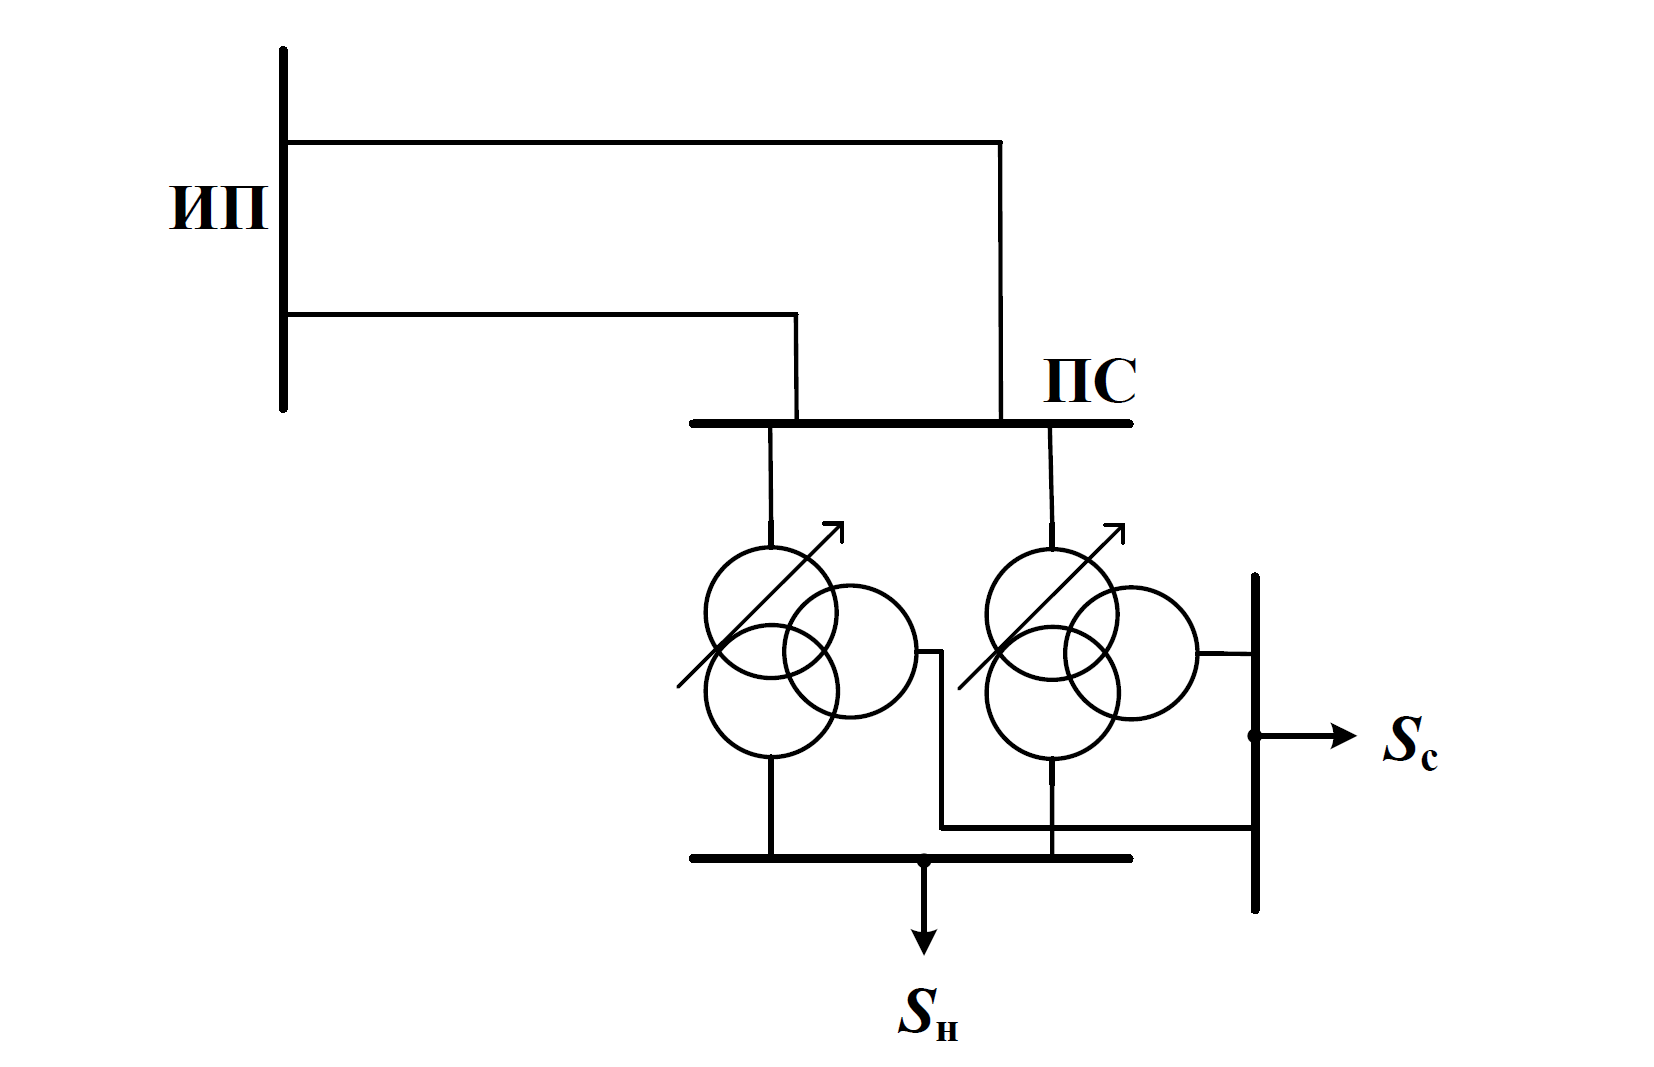
\includegraphics[width=0.9\textwidth]{inc/img/ish_dannie}
	\caption{Схема сети}
	\label{fig:scheme}
\end{figure}

Номинальное напряжение сети $U_{\text{ном}}$, марка проводов и длина линии $L_{\text{ИП-ПС}}$ от источника питания (ИП) до ПС, трансформаторы, установленные на ПС, приведены в табл.~\ref{tab:tabl1}. На шинах ИП района в режиме наибольших нагрузок обеспечивается напряжение, указанное в табл.~\ref{tab:tabl1} , а в режиме наименьших нагрузок 97 \% от номинального. Низшее напряжение на ПС составляет 10 кВ.

Мощность нагрузок на шинах низшего и среднего напряжений (НН и СН) ПС в режиме наибольших нагрузок ($P_{\text{н}}$ и $P_{\text{с}}$), наименьшая нагрузка (относительное снижение нагрузки $\alpha$) и число часов использования наибольших нагрузок $T_{\text{нб}}$ приведены в табл.~\ref{tab:tabl2}.

\renewcommand{\thetable}{\arabic{table}}
\begin{table}[H]
	\caption{Исходные данные для расчета (часть 1)}
	\begin{tabular}{|r|c|c|c|l|}
		\hline
		$U_{\text{ном}}$ , кВ & $U_{\text{ИП}}$, \% & $L_{\text{ИП-ПС}}$ & Марка провода & Трансформатор \\
		\hline
		110 & 113 & 84 & АС 150/24 & ТДТН-40000/110/35 \\
		\hline
	\end{tabular}
	\label{tab:tabl1}
\end{table}

\begin{table}[H]
	\caption{Исходные данные для расчета (часть 2)}
	\begin{tabular}{|r|c|c|c|c|l|}
		\hline
		$P_{c}$, кВт & $cos\varphi_c$ & $P_{\text{н}}$, кВт & $cos\varphi_{\text{н}} / tg\varphi_{\text{н}} $ & $\alpha$, отн. ед. & $T_{\text{нб}}$, ч/год \\
		\hline
		33000 & 0,82 & 22880 & - / 0,44 & 0,4 & 6820 \\
		\hline
	\end{tabular}
	\label{tab:tabl2}
\end{table}

По табл. 3.5 и 3.8 \cite{файбисович} определяем необходимые для расчета исходные данные по проводу АС 150/24 и сводим их в табл.~\ref{tab:tabl3}

\begin{table}[H]
	\caption{Расчетные данные сталеалюминевого провода АС 150/24}
	\begin{tabular}{|c|c|c|}
		\hline
		Номинальное сечение & Диаметр провода  & Активное сопротивление \\
		(алюминий/сталь) & $d_{\text{пр}}$, мм & постоянному току при \\
		провода, $\text{мм}^2$ & & температуре 20 $^{\circ}$C \\
		 & & $R_0$, Ом/км \\
		\hline
		150/24 & 17,1 & 0,204 \\
		\hline
	\end{tabular}
	\label{tab:tabl3}
\end{table}


\renewcommand{\thefigure}{\arabic{chapter}.\arabic{figure}} % возвращаем нормальную нумерацию картинок
\renewcommand{\thetable}{\arabic{chapter}.\arabic{table}} % возвращаем нормальную нумерацию таблиц

%%% Local Variables: 
%%% mode: latex
%%% TeX-master: "rpz"
%%% End: 